\documentclass{article}

\usepackage{minted}
\usepackage[most]{tcolorbox}
\usepackage{geometry}
\usepackage{enumitem}
\usepackage{hyperref}
\usepackage{hyperref}
\usepackage[parfill]{parskip}
\usepackage{wrapfig}
\usepackage{accsupp}

\geometry{margin=0.8in}
\definecolor{lightgreen}{rgb}{0.56, 0.93, 0.56}
\definecolor{moonstoneblue}{rgb}{0.45, 0.66, 0.76}
\definecolor{magenta}{rgb}{0.8,0.66,0.76}
\begin{document}
\BeginAccSupp{}
\begin{flushright}
Computational Biology ~\\
Tufts University Bio 35 ~\\
Fall 2021 ~\\ ~\\
\end{flushright}
\begin{center}{\textbf{\Large{Spotlight 6: Swanne Gordon}}}\end{center}

\textit{Please note that in general I have taken/adapted the words of our Spotlight subjects from their own websites to describe their work. I have done this in an effort to maintain accuracy in describing their research programs. Please do not copy paste text from their papers/websites in your assignments!}

\begin{wrapfigure}{L}{0.16\textwidth}
\begin{center}
 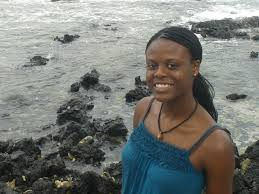
\includegraphics[width=0.17\textwidth]{images/swanne-gordon.jpeg}
 \end{center}
\end{wrapfigure}
~\\ As part of our unit on adaptive evolution and population genetics, we are going to explore the work of Swanne Gordon. Prof. Gordon's lab is built around the underlying question: \textit{why is there diversity in nature, and how is it maintained}? She uses a multidisciplinary approach to study the selective forces maintaining colour polymorphism in the aposematic wood tiger moth \textit{Arctia plantaginis}. She also carries out experimental evolution studies in Trinidadian guppies \textit{Poecilia reticulata}, to elucidate the mechanisms behind rapid adaptation to environmental change. She is an Assistant Professor at Washington University in St Louis.
~\\

Please read the following articles about Prof. Gordon and her research: 
\begin{enumerate}
\item \texttt{\href{https://www.sciencedaily.com/releases/2015/09/150914215611.htm}{https://www.sciencedaily.com/releases/2015/09/150914215611.htm}}
\item \texttt{\href{https://www.nature.com/articles/s41559-021-01415-1}{https://www.nature.com/articles/s41559-021-01415-1}}
\end{enumerate}

\subsubsection*{Written Assignment} 
After reading about Swanne Gordon please write a reflection (max one page) on what you discovered. You might wish to address some of the following: 

\begin{enumerate}
\item What was most interesting to you in reviewing these resources?
\item What did you learn from these resources about polymorphism or biodiversity? How might computational tools help us to identify biodiversity loss or study the mechanisms for biodiversity maintenance?
\item What new questions do you have after reviewing these resources?
\item What do these resources tell you about the types of people that do computational biology, or their motivations?
\end{enumerate}

\EndAccSupp{}
\end{document}
